\section{Structure}
\label{sec:problem_structure}
The class diagram is based on the classes and events, which is described earlier in chapter \ref{cap:classesevents}. The class \class{person} aggregates a role. The role class itself is removed since only \class{\client[]} inherited from it. \class{\staff[]} inherits from \class{\client[]} and \class{\admin[]} inherits from \cl{\staff[]}. Alternatively the role pattern could have been used. This prescribes that \class{\client[]}, \class{\staff[]}, and \class{\admin[]} all would have been a subclass of \textit{\cl{role}}  \cite[p. 80]{roedeaalborg}. We consider that it makes more sense that they inherited from each other, because they have a lot of shared properties and privileges.
%since all the privileges \class{\staff[]} has the \class{\admin[]} has as well. Same applies for \class{\staff[]} and \cl{\client[]}.  

For the class person different relations appear depending on his role. 
\begin{itemize}
\item \cl{\client[]s} can subscribe to \cl{problems}.
\item \class{\staff[]} can be assigned to \class{problems} and \class{\staff[]} belongs to a department. 
\item \class{\admin[]} does not have any relations. But is necessary for administration of users.  
\end{itemize}

A \problem[] consist of none or many \textit{comments}, none or many \textit{solutions} and, one or many \textit{tags}. A \cl{tag} belongs to a category and a \class{category} belongs to a \class{department}.  The class diagram is illustrated at figure \ref{fig:pdaclassdiagram}

\begin{figure}
\begin{center}
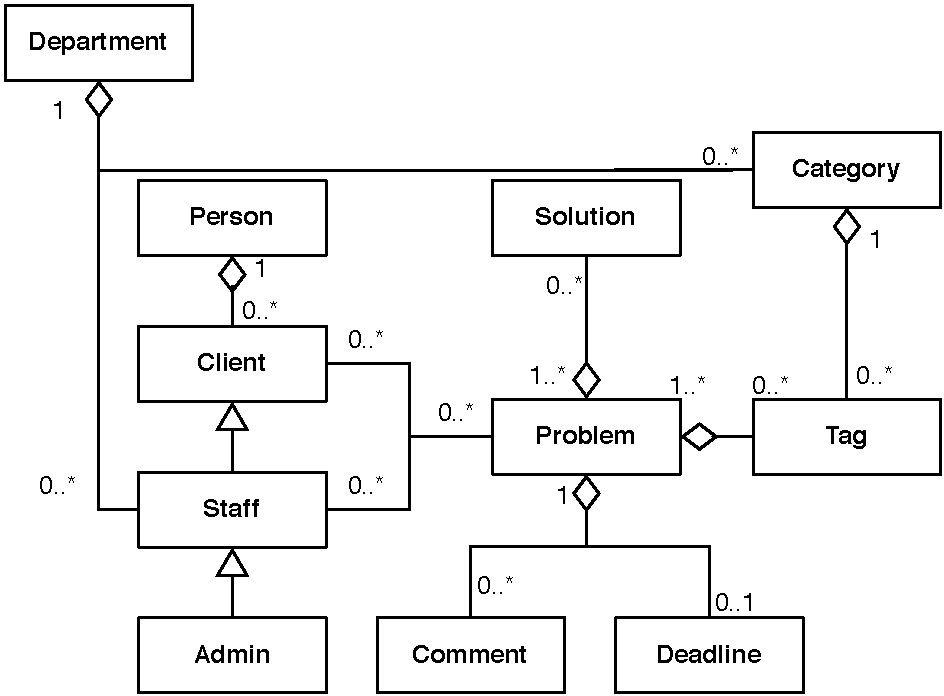
\includegraphics[scale=0.6]{input/problem_domain_analysis/newest_class_diagram.pdf}
\morscaption{Class diagram}
\label{fig:pdaclassdiagram}
\end{center}
\end{figure}